\chapter{Matrix calculations - Quadratic placement by GR633}
\graphicspath{{figures/}}
\section{a) Explain how to find the positions of the free cells that minimize the total wire length}
The total square wire length is given by \autoref{matrix:Jk}.
\begin{flalign}
J_K=\sum_{k=1}^K\left[(x_{I(k)}-x_{J(k)})^2+(y_{I(k)}-y_{J(k)})^2\right] \label{matrix:Jk}
\end{flalign}
where $x_{I(K)}$ is the position where the wire start and $x_{J(K)}$ is the position where the wire ends. Likewise with y. 

By defining the position of the free cells, $x_{free}$, as $[x_1,x_2,...,x_n]^T$ and the fixed cells, $x_{fixed}$, as $[x_{n+1},...,x_N]^T$, x can be defined as $[x_{free}^T, x_{fixed}^T]^T$ and similarly with y.

The matrix, A, describes which wire connects the start cell, I(k), to the end cell, J(k). It can then be shown that
\begin{flalign*}
x_{I(k)}-x_{J(k)}=A_kx
\end{flalign*}
as $A_{kj}$ is -1 if wire $k$ goes from cell $j$, 1 if wire $k$ goes to cell $j$ or 0 otherwise.

A simple example can be seen in \autoref{matrix:A}.
\begin{flalign}
&A_1=[-1, 0, 0, 1], x=[x_1, x_2, x_3, x_4]^T, \text{from cell 1 to cell 4} \notag \\
&A_1x=x_4-x_1\label{matrix:A}
\end{flalign}

To get the same expression as \autoref{matrix:Jk} the term needs to be squared. This is similar to squaring the norm of $Ax$. The cost function can thus be rewritten to be \autoref{matrix:AxAy}.
\begin{flalign}
J_K=\left(||Ax||_2^2+||Ay||_2^2\right) \notag \\
J_K=\left(||A[x_{free}^T, x_{fixed}^T]^T||_2^2+||A[y_{free}^T, y_{fixed}^T]^T||_2^2\right) \label{matrix:AxAy}
\end{flalign}

The cost function is similar to the least square approximation as the function needs to be minimized by selecting $x_{free}$ and $y_{free}$ that gives the least squares.

\section{b) Determine the optimal quadratic placement for a specific set of cells and interconnect topology.}
\autoref{matrix:AxAy} is minimized using the CVX toolbox in matlab c.f. matrix_hw_GR633.m except the norm isn't squared in the matlab program as it gave an error with the CVX toolbox. This isn't an issue as the minimizer will be the same.

\begin{figure}[htbp]
\centering
\begin{subfigure}{0.45\textwidth}
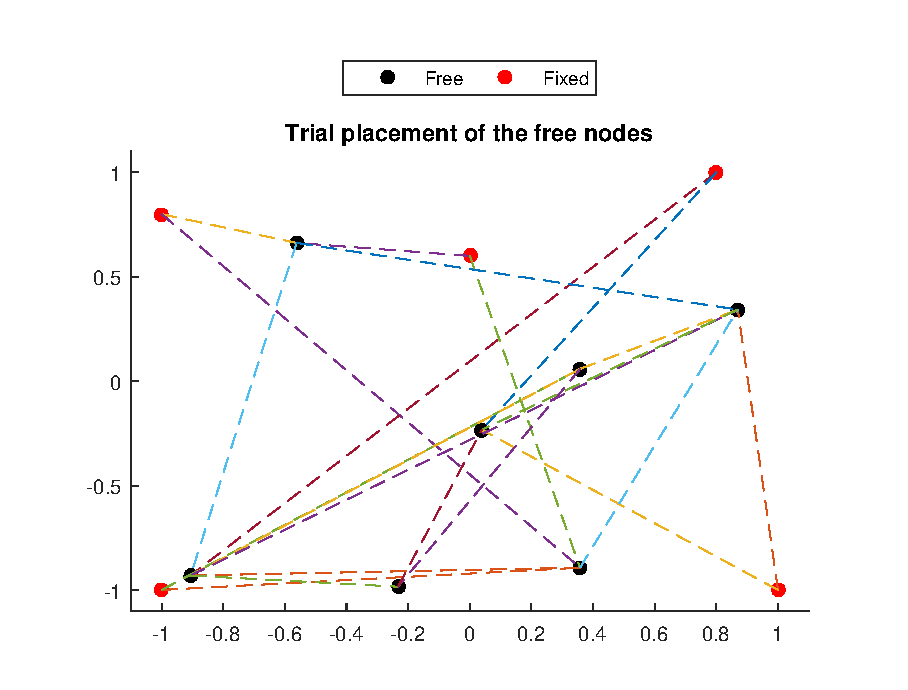
\includegraphics[width=\textwidth]{matrixrand}
\caption{Plot of randomly selected free cells.}
\end{subfigure}
\begin{subfigure}{0.45\textwidth}
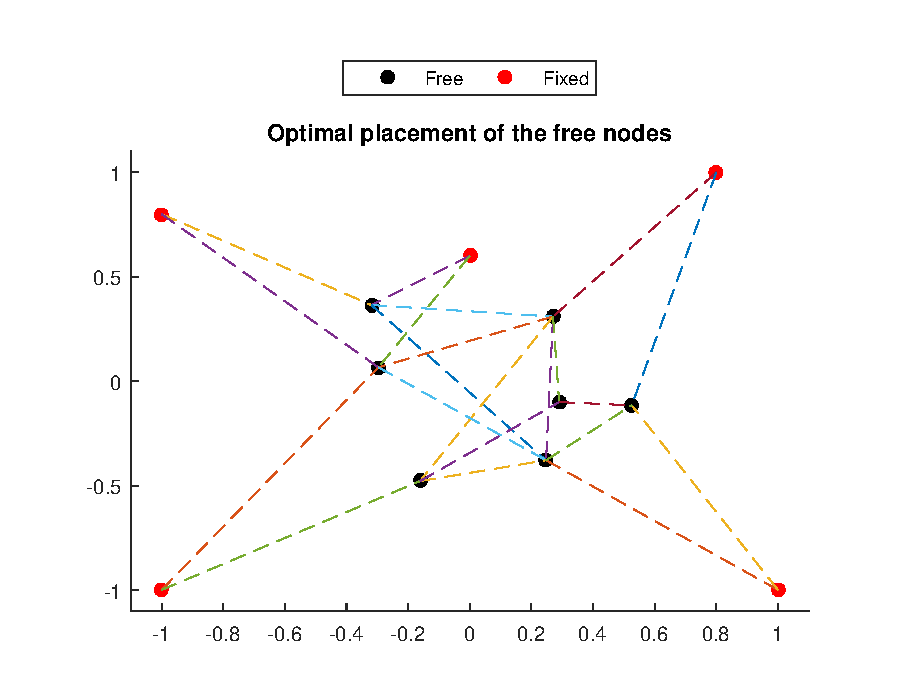
\includegraphics[width=\textwidth]{matrixopt}
\caption{Plot of free cells selected by minimizing \autoref{matrix:AxAy}.}
\end{subfigure}
\caption{Plot of the fixed and free cells incl. their wiring.}
\label{matrix:fig}
\end{figure}

On \autoref{matrix:fig} the fixed and free cells are seen where they're randomly selected or optimized. Since they're connected to each other and/or the fixed cells it makes sense that the optimized cells are closer to the center of the fixed cells than when randomly selected.